\section{Method}\label{sec:method}
We propose \textbf{Lo}RA-\textbf{F}ine-\textbf{T}uning-aware \textbf{Q}uantization (LoftQ), a quantization framework for LLMs. It alternatively applies quantization and low-rank approximation to approximate original pre-trained weights. 
This quantization framework provides a promising initialization for LoRA fine-tuning, which alleviates the quantization discrepancy in QLoRA and improves generalization in downstream tasks significantly.

\subsection{LoRA-Aware Quantization}
% Given an $N$-bit low-precision weight $Q \in \RR_{N}^{d_1 \times d_2}$ that is quantized from a high-precision weight $W \in \RR^{d_1 \times d_2}$, we add low-rank adapters $A \in \RR^{d_1 \times r}$ and $B \in \RR^{d_2 \times r}$ to it. 
% Usually, these low-rank adapters are initialized by \ref{eq:lora_init}. Such an initialization, $Q + AB^{\top}$, however, no longer aligns with the high-precision pre-trained weights due to the quantization error. This misalignment often leads to severe performance decrease during fine-tuning, especially in low-bit situation (see Section \ref{sec:experiment}).
We use an $N$-bit quantized weight $Q \in \RR_{N}^{d_1 \times d_2}$ and low-rank approximations $A \in \RR^{d_1 \times r}, B \in \RR^{d_2 \times r}$ to approximate the original high-precision pre-trained weight $W \in \RR^{d_1 \times d_2}$ as the initialization of LoRA fine-tuning.
Specifically, before fine-tuning, we initialize the network by minimizing the following objective:
\begin{align}
\label{eq:optimization}
   \underset{Q, A, B}{\min}  \norm{W - Q - AB^{\top}}_{F},
\end{align}
where $\norm{\cdot}_{F}$ denotes the Frobenious norm. This objective in \eqref{eq:optimization} takes LoRA fine-tuning into consideration by jointly optimizing the initial values of the quantized backbone $Q$ and low-rank adapters $A, B$.
% The optimal $Q$ is the frozen backbone and the optimal $A, B$ servers as the low-rank adapters in LoRA fine-tuning. 
Contrarily, practitioners typically convert the pre-trained weight $W$ into a quantized weight $Q$ outright, neglecting the subsequent LoRA fine-tuning process. This oversight leads to notable performance degradation in downstream tasks arising from the quantization discrepancy.
%This lack of consideration results in a substantial performance drop on downstream tasks due to the quantization error.

% Taking LoRA fine-tuning into consideration, we introduce low-rank approximation  $A \in \RR^{d_1 \times r}$ and $B \in \RR^{d_2 \times r}$. During LoRA initialization, our goal is to consider the quantization and low-rank approximation as a unified entity and align it with the original high-precision weights. 

% We solve the optimization in \eqref{eq:optimization} by combining quantization and singular value decomposition (SVD).

\subsection{Alternating Optimization}
\label{sec:alternating_optimization}
We solve the minimization problem in \eqref{eq:optimization} by alternating between quantization and singular value decomposition (SVD). To begin with, we set $A_0$, and $B_0$ equal to 0.

\noindent \textbf{Quantization}. At the $t$-th step, we quantize the difference between the original pre-trained weight $W$ and the low-rank approximation $A_{t-1}B_{t-1}^{\top}$ from the last step to obtain the quantized weight $Q_{t}$ by 
\begin{align}
\label{eq:quant_method}
    Q_t = q_N(W - A_{t-1}B_{t-1}^{\top}),
\end{align}
where $q_N(\cdot)$ maps a high-precision weight matrix to a quantized matrix.

We remark that our algorithm is compatible with different quantization functions $q_N(\cdot)$. We apply NF4 and the uniform quantization in Section \ref{sec:experiment} as examples. We also remark that $Q_t$ is not an exact solution of the minimization in \eqref{eq:optimization}, given the fixed $A_{t-1}B_{t-1}^{\top}$, but it is an efficient approximation.

\noindent \textbf{SVD}. After obtaining the $t$-th quantized weight $Q_t$, SVD is applied to the residual of the quantization denoted by $R_t = W - Q_t$ by
\begin{align}\label{eq:residual}
R_t =\sum_{i=1}^d\sigma_{t, i} u_{t, i} v_{t,i}^{\top},
\end{align}
where $d = \min\{d_1,d_2\}$, $\sigma_{t, 1} \geq \sigma_{t, 2} \geq ... \geq \sigma_{t, d}$ are the singular values of $R_t$, $u_{t, i}$'s and $v_{t, i}$'s are the associated left and right singular vectors of $R_t$. We then obtain a rank-$r$ approximation of $R_t$ by $A_{t}B_{t}^{\top}$, where
\begin{align}
\label{eq:svd}
A_t &= [\sqrt{\sigma_{t, 1}} u_{t, 1},...,\sqrt{\sigma_{t, r}}u_{t, r}],\nonumber\\
B_t &= [\sqrt{\sigma_{t, 1}} v_{t, 1},...,\sqrt{\sigma_{t, r}}v_{t, r}].
\end{align}

We summarize our method in Algorithm \ref{alg:alter}. It is worth noting that $T=1$ is a special case where $Q_1$ is the exact quantized weight obtained by QLoRA, and low-rank approximations $A_1, B_1$ are obtained by the SVD of the quantization residual $W - Q_1$. $T=1$ is sufficient to mitigate the quantization discrepancy, and alternating optimization helps to find a closer initialization to the pre-trained weight $W$, which further improves the performance (see Section \ref{fig:num_iter}).


\begin{algorithm}
    \caption{{\OurAlg}}\label{alg:alter}
    \begin{algorithmic}[1]
        \INPUT {Pre-trained weight $W$, target rank $r$, $N$-bit quantization function $q_N(\cdot)$, alternating step $T$}
        \STATE {Initialize $A_0 \leftarrow 0, B_0 \leftarrow 0$}
        \FOR {t = $1$ to $T$}
            \STATE {Obtain quantized weight $Q_t \leftarrow q_N(W - A_{t-1}B_{t-1}^{\top})$}
            \STATE {Obtain low-rank approximation $A_t, B_t \leftarrow \text{SVD}(W - Q_t)$} by \eqref{eq:svd}{}
            
        \ENDFOR
        \OUTPUT {$Q_T, A_T, B_T$}
    \end{algorithmic}
\end{algorithm}


% Figure \ref{fig:optimization_singular_values} shows that the residual $R$ in \eqref{eq:residual} has only a few large singular values, demonstrating its low-rank characteristics and indicating the low-rank approximation is efficient.

% We remark that our method is applicable to different types of quantization methods such as NF4 and uniform. 
% the quantization function $q_N(\cdot)$ in \eqref{eq:quant_method} is not limited to some specific ones, such as NF4, the one used in QLoRA. Instead, we can apply various quantization method, for example, uniform quantization. The experiments in Section \ref{sec:experiment} show the success of our method in a variety of quantization methods. 

We remark that the computational cost of {\OurAlg} is negligible because it is applied to individual weight matrices and therefore can be executed in parallel. We also remark one can apply {\OurAlg} only once to a pre-trained model and reuse the initialization obtained by {\OurAlg} for different downstream tasks.
% For example, it takes less than an hour to apply {\OurAlg} to LLAMA-2-13b on CPU.

% From Figure \ref{fig:alter_loss}, we notice the alternating method successfully further reduce the discrepancy between the pre-trained weights and the initialization. 

% \begin{figure}[htb!]
% \centering
% \begin{subfigure}{0.49\columnwidth}
%     \centering
%     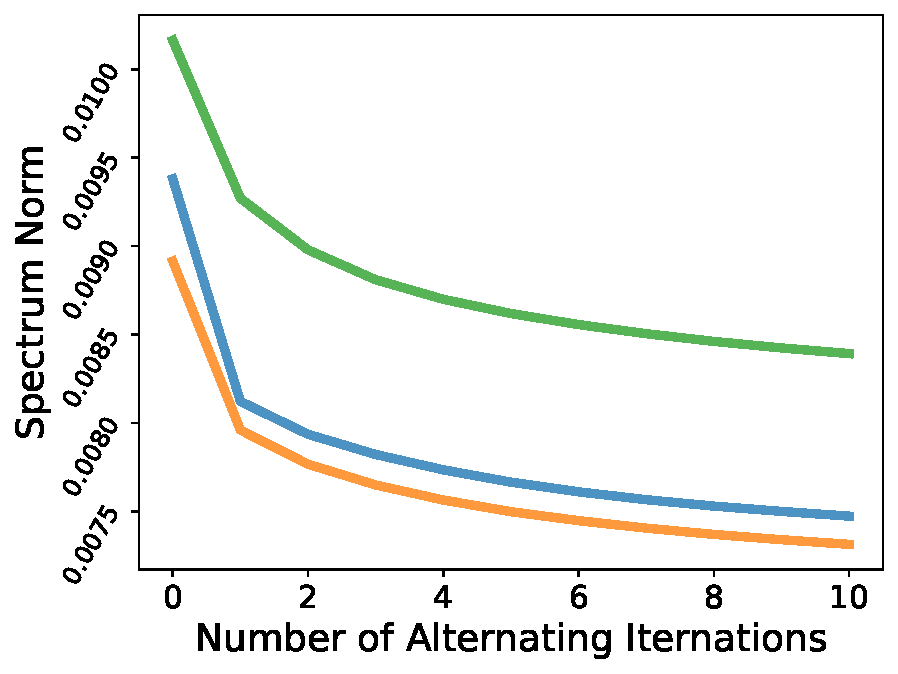
\includegraphics[width=1.0\textwidth]{figures/alter_loss_bart.pdf}
%     \caption{$W_{\rm{fc1}}$ of Layer 0 of BART-large}
%     \label{fig:alter_loss}
% \end{subfigure}
% \begin{subfigure}{0.49\columnwidth}
%     \centering
%     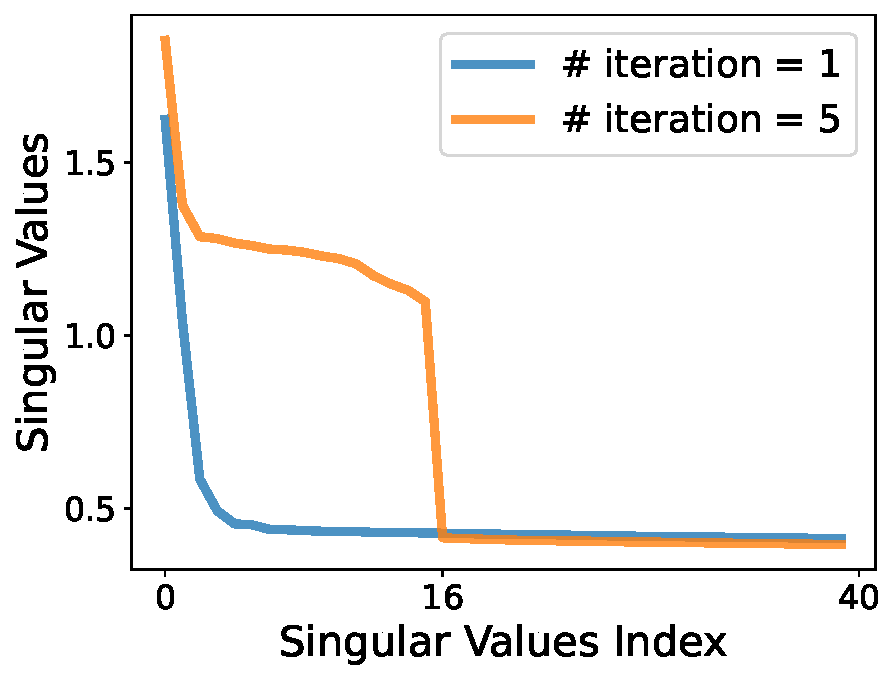
\includegraphics[width=1.0\textwidth]{figures/bart-decoder-fc2-nf2-lora.pdf}
%     \caption{$W_{\rm{fc2}}$ of Layer 2 of BART-large}
%     \label{fig:optimization_singular_values}
% \end{subfigure}
% \caption{
% Illustration of the effectiveness of alternative optimization. \textbf{Left:} Alternative optimization successfully reduces the spectral norm of the difference between pre-trained weights and hybrid approximation. \textbf{Right:} The residual only displays few large eigenvalues where the number of large eigenvalues equals our designated rank. This low rank approximation for the residual is efficient.
% % Importance scores are calculated when compressing DeBERTa-base on SST-2 at the 3156\textsuperscript{th} step. \textit{Layer 7, Query} indicates the matrix is from the query matrix at the 7th layer.
% }
% \vspace{-1mm}
% \label{fig:optimization}
% \end{figure}

\subsection{Applying to LoRA Fine-tuning}
We store the $Q_T \in \RR_N^{d_1 \times d_2}$ obtained by {\OurAlg} using an integer matrix $M$ by \eqref{eq:quant} and a lookup table $\cT$ by \eqref{eq:lookup_table}. 
% The integer matrix $M$ serves as the frozen backbone weight in LoRA fine-tuning. We initialize the low-rank adapter of LoRA with $A_T, B_T$ obtained by {\OurAlg}.
We initialize the backbone with the integer matrix $M$ and initialize the low-rank adapters with $A_T, B_T$ obtained by {\OurAlg}. 

During LoRA fine-tuning, we freeze the integer weight $M$ and optimize the low-rank adapters with an efficient optimization algorithm, e.g., AdamW \citep{loshchilov2017decoupled}.
% We apply $Q_T$ and $A_T, B_T$ obtained by {\OurAlg} as the initialization of LoRA fine-tuning. $Q_T$ serves as the frozen backbone weight, and $A_T, B_T$ are the initial low-rank adapter.
% In LoRA fine-tuning, we fix the quantized weights $Q_T$ and update low-rank adapters starting from $A_T, B_T$ by some SGD-type optimization algorithm.
% In LoRA fine-tuning, we fix the integer weight $M$ and update low-rank adapters $A, B$ starting from $A_T, B_T$ by some SGD-type optimization algorithm.
% In forward propagation, the integer weight $M$ is temporarily dequantized to a simulated high-precision weight by its lookup table when it is engaged in matrix multiplication.
In forward propagation, the integer weight $M$ is temporarily dequantized to the simulated high-precision weight $Q_T$ by its lookup table, as described in \eqref{eq:dequant}.
% Such temporary dequantization does not cost additional storage when the linear transformation has completed.
% rendered to high precision just in time, or use special low bit matrix multiplication code such as \texttt{bitsandbytes}~\cite{dettmers2022llmint8,dettmers2022optimizers}.
In back propagation, gradients and optimizer state are only related to low-rank adapters $A, B$, which reduces considerable training cost. 
